\documentclass{article}
\usepackage{tikz}
\usepackage{blkarray}
\usepackage{amsmath}
\usetikzlibrary{arrows}
\usetikzlibrary{calc}
\usepackage{amsmath}% http://ctan.org/pkg/amsmath
\usepackage{kbordermatrix}% http://www.hss.caltech.edu/~kcb/TeX/kbordermatrix.sty
\begin{document}

\section*{Stochastic Simulation}

The data is simulated from a spatial markov chain with variable transition probabilities. Participants alter between three possible states: ‘roam’, ‘check phone’ and ‘conversation’. The probability of transition between the states depends not only on the location of the participant relative to other participants, but also the ‘fame’ score and specialization field of nearby participants. 
This way, the probability of engaging in conversation instead of checking one’s phone is higher if in the vicinity of a famous participant from the same specialization. We denote $f_{ij}(\theta,\phi)$ as the probability of transitioning from state $i$ to $j$, given nearby location information $\phi$ and parameters $\theta$.

We run the model over a variety of parameters, and during the SC14 conference, hope to train the model with real-world data gathered from attendees. 

\begin{figure}[hptb!]
\centering
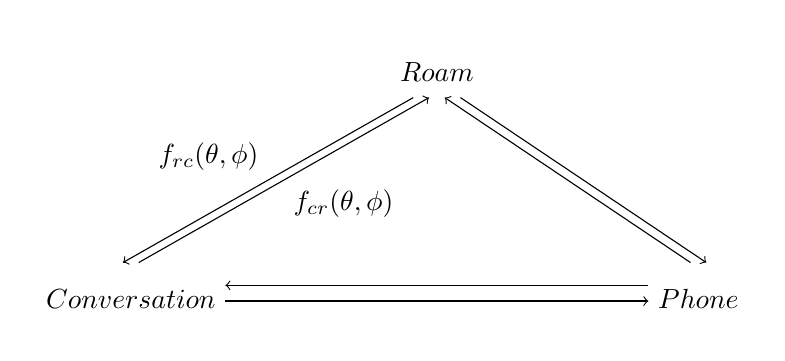
\begin{tikzpicture}[description/.style={fill=white,inner sep=2pt}]
\usetikzlibrary{arrows,decorations.pathmorphing,backgrounds,positioning,fit,matrix}
\matrix (m) [matrix of math nodes, row sep=6em,
column sep=6em, text height=3ex, text depth=0.5ex]
{ & Roam & \\
Conversation & &  Phone \\ };
\path[->] ($(m-2-3.north)+(-0.1,0)$) edge ($(m-1-2.south)+(+0.1,0)$);
\path[<-] ($(m-2-3.north)+(+0.1,0)$) edge ($(m-1-2.south)+(+0.3,0)$);

\path[->] ($(m-1-2.south)+(-0.3,0)$) edge node[above left] {$f_{rc}(\theta,\phi)$} ($(m-2-1.north)+(-0.1,0)$);
\path[<-] ($(m-1-2.south)+(-0.1,0)$) edge node[below right] {$f_{cr}(\theta,\phi)$} ($(m-2-1.north)+(+0.1,0)$);
;
\path[->] ($(m-2-1.east)+(0,-0.1)$) edge ($(m-2-3.west)+(0,-0.1)$);
\path[<-] ($(m-2-1.east)+(0,+0.1)$) edge ($(m-2-3.west)+(0,+0.1)$);
\end{tikzpicture}
\caption{A graph illustrating the transition states of the model. The functional notation is only shown twice as an example} \label{fig:diagram}
\end{figure}
 
 
The form of the transitional probabilities is written out in the matrix below:

  \text{Transition Matrix} = \kbordermatrix{
    & r& c& p& \\
r& f_{rr}(\phi,\theta) & f_{rc}(\phi,\theta)& f_{rp}(\phi,\theta)\\
 c& f_{cr}(\phi,\theta)& f_{cc}(\phi,\theta)& f_{cp}(\phi,\theta)\\
    p & f_{pr}(\phi,\theta)& f_{pc}(\phi,\theta)& f_{pp}(\phi,\theta)\\
  }


\end{document}

